
\documentclass[journal]{IEEEtran}

\usepackage{graphicx}
\usepackage[utf8]{inputenc}
\usepackage{algorithm}
\usepackage{algorithmic}
\usepackage{amsmath}
\usepackage{amssymb}
\usepackage{caption}

%\usepackage[noend]{algpseudocode}

%\usepackage[noend]{algpseudocode}

%\restylefloat{algorithm}



\begin{document}
 
\title{\textbf{handling learnability imbalance in multiclass-classification}}



\author{Theodor Peifer
        \linebreak
        email: thp7219@thi.de
        \linebreak
        Technische Hochschule Ingolstadt
}



\maketitle


\begin{abstract}
Neural Networks have proven themselves to be powerful classification
tools by solving problems in a range of domains with high accuracy.
Yet this accuracy is never evenly distributed across all classes (i.e. the categories the model has to classify between), which means that the true-positive rates of each class separately are different.
This can happen even in balanced datasets since some classes are more difficult to learn by the model than others (this phenomenon is further referred to as \emph{learnability-imbalance}).
A common way to address this problem is to give a weight to the error function for each class to penalize losses of certain classes higher or lower.
This research will address the determination of such weights to counteract the learnability-imbalance in balanced datasets using previously calculated evaluation scores.
Therefore the goal is to find methods to lower the variance of the true positive rates of each class.
\end{abstract}


\section{Introduction}
A frequent problem in classification appears when working with datasets that have an unequal amount of samples per class and are therefore called a \emph{class imbalanced} datasets. %, where \emph{classes} describe the categories which the model has to classify.
Since there will be some classes, that have less elements for the model to learn from, their features will be harder to extract what finally will result in a lower true positive rate, i.e. a per-class accuracy [1].
Thus, the consequence of having different class sizes can be described as having a \emph{learnability imbalance} in the dataset, since some classes are more difficult to learn that others.
%Classes with less element are harder to learn, which won't only result in big differences in the true positive rates [1] of the individual classes but also in a lower, overall accuracy.
%In order to prevent this, it is common to weight the error function [1] according to the size of each class, i.e. the number of samples it contains.
%Therefore, for every class there is a weight, which is greater the fewer elements it contains and that gets multiplied with the loss produced by its samples. % "Therefore" wrong
%Since the aim of a neural network is to minimize the overall loss and samples from a smaller class will produce a higher error, they will have a higher impact on the learning process in order to compensate for the different class sizes.

% , samples from that produce a high loss will have a higher impact on the learning process.
% This can prevent the model from learning the patterns of a class with less element worse than others.
% With the evaluation a set of true positive rates can be calculated for each class which reveals what classes are more difficult to learn by the model and should have received a higher weight. 

But such learnability differences can appear also in balanced datasets for a variety of reasons, e.g. when the quality of the data of a class is lower than the rest of the data. % or when the classes come not from the distributions. 
A second reason, that this research will be focusing on, is that when some classes are similiar, % "similiar objects"?
the model can confuse their samples with each other more easily which will often result in a lower accuracy of those classes.
%This issue is an inevitable product of every normal classification.

%This issue is a light version of the imbalanced dataset problem and the inevitable product of every normal classification. 
Even though this issue is an inevitable product of every normal classification, in most cases the learnability difference of the classes is either low or not from great interest.
But there can be more extreme cases in which a model needs to produce fair and unbiased results using a dataset that has an obvious learnability imbalance. 
An example for that is \emph{name-ethnicity classification}, where a model predicts the ethnicity of a name only by its letters [5]. 
Nationalities that use the same language and therefore have similiar names (e.g. \emph{british} and \emph{american}) result in a lower accuracy (see figure 1).
Thus, when a model that is trained on such a dataset is used, e.g. for social science experiments, it can lead to unfair results and wrong interpretations. 

\begin{figure}[h!]
        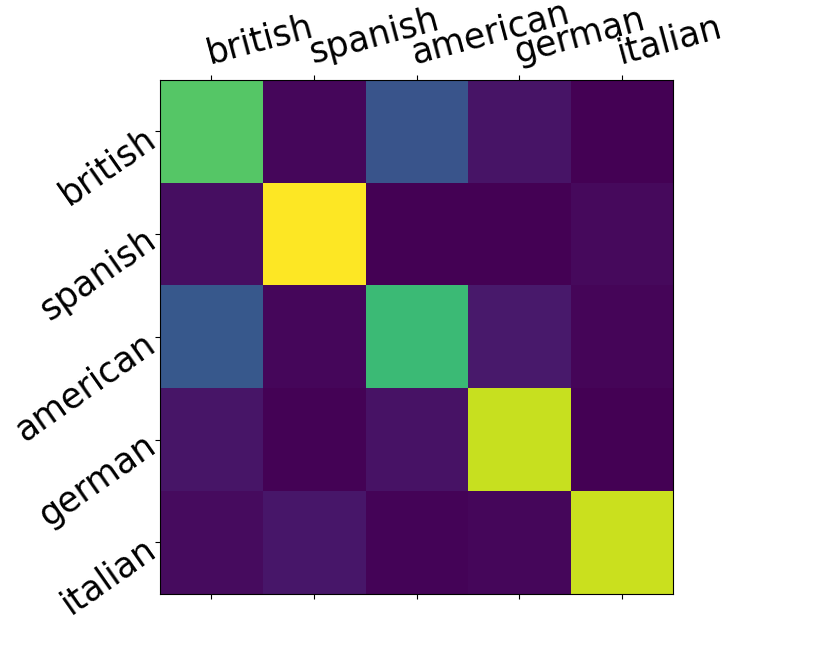
\includegraphics[width=\linewidth]{images/Figure_1.png}
        \caption{A confusion matrix representing the true positive distribution of the name-nationality dataset produced by a recurrent neural network and the confusion of british and american names}
        \label{fig:tp_scores}
\end{figure}

Another dataset that is a good showcase for the learnability imbalance is the CIFAR-10 [2] dataset (32$\times$32 RGB images of ten different classes) because it also contains similiar classes such as \emph{dog} and \emph{cat}.
%Another dataset that is a good showcase for the learnability imbalance is the CIFAR-10 [2] dataset because in the 10 different classes which consist of 32x32 pixel images, there are also similiar ones such as \emph{dog} and \emph{cat}.
The CIFAR-10, a name-nationality and a further tabular dataset will be used for experiments in order to find methods for minimizing such variances in the evaluation scores.

%\begin{figure}[h!]
%        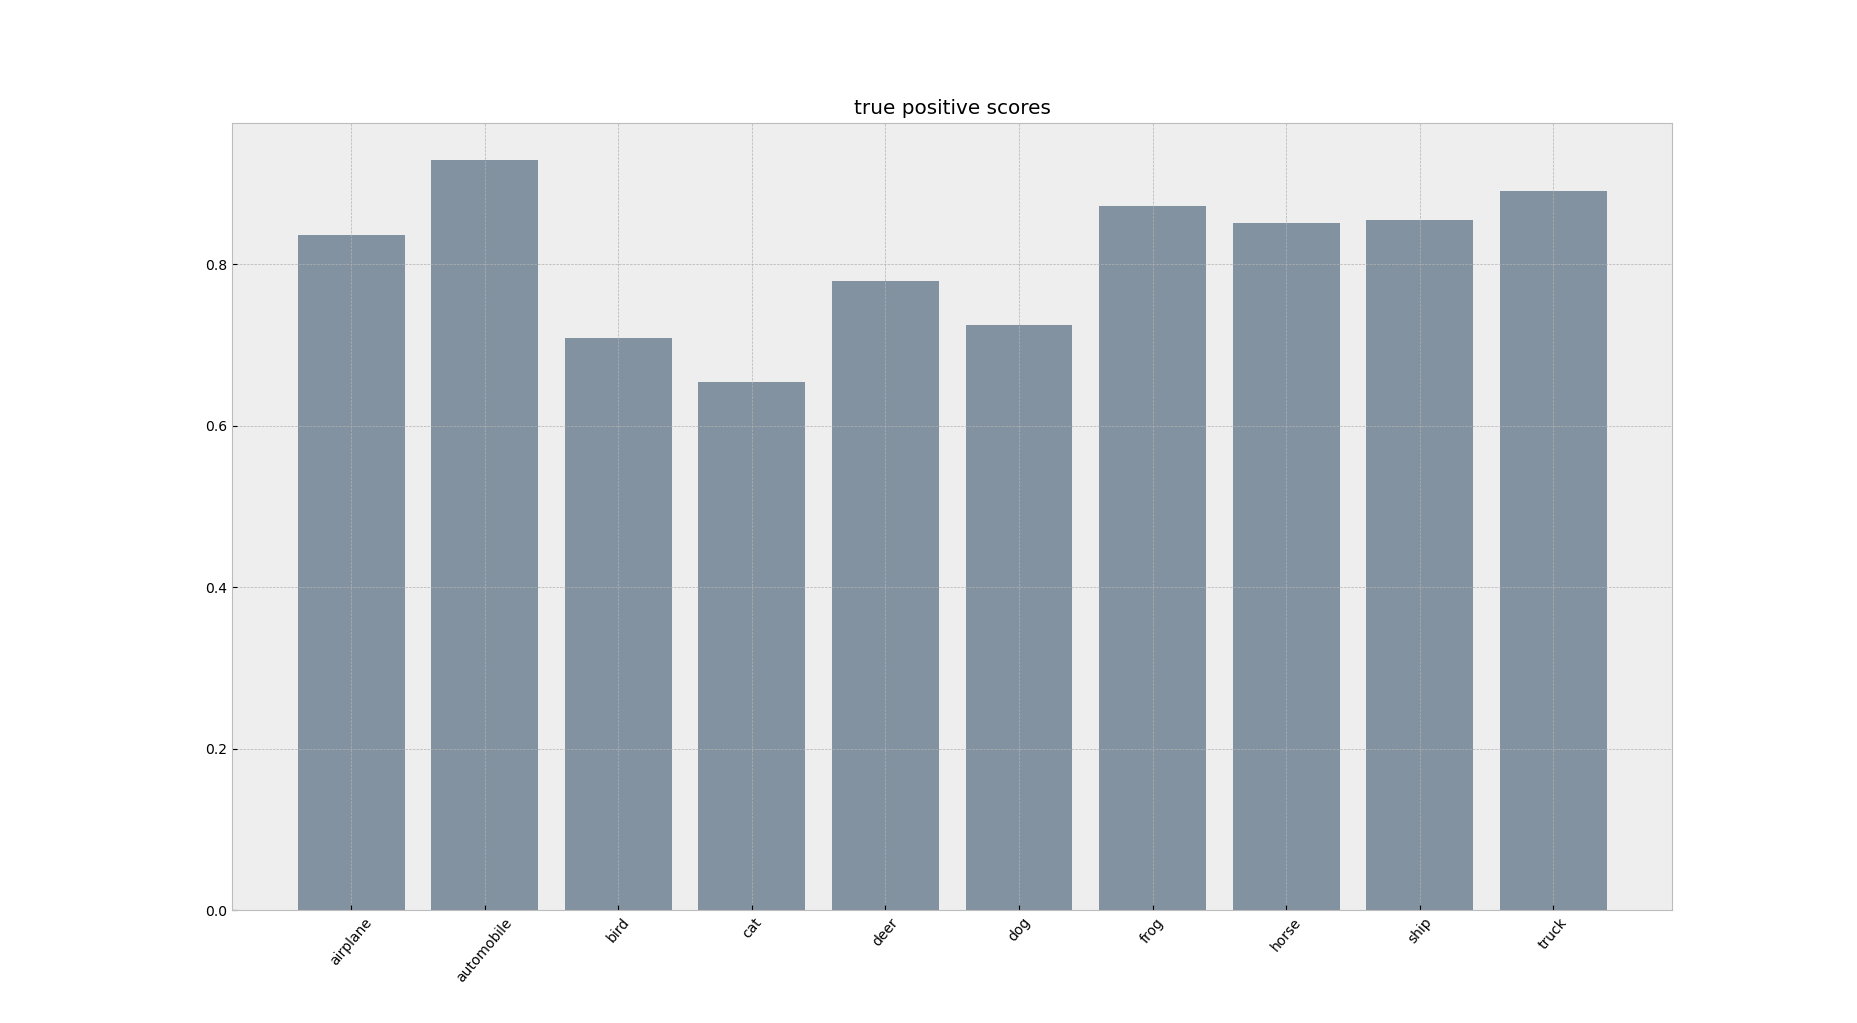
\includegraphics[width=\linewidth]{images/cifar10_tp_scores.png}
%        \caption{true positive scores of a model trained on the CIFAR-10 dataset}
%        \label{fig:tp2_scores}
%\end{figure}

%---> When working with such datasets the learnability differences of the individual classes are mostly only identifiable after the model has been trained and evaluated normally.
%---> A confusion matrix or the calculation of the true positive rates then reveal what classes where learned the best and which should have received a higher weight. 

To figure out such methods one should first go back to the class imbalance problem because there are already solutions existing.
One of which is to weight the error function [1] according to the size of each class, i.e. the number of samples it contains.
Therefore, there is a weight assigned to every class, which is greater the fewer elements it contains and that gets multiplied with the loss produced by its samples. % "Therefore" wrong
%Since the aim of a neural network is to minimize the overall loss and samples from a smaller class will produce a higher error, they will have a higher impact on the learning process in order to compensate for the different class sizes.
That will cause, that samples from a smaller class will produce a higher error and, since the aim of a neural network is to minimize the error [4], will receive a higher focues in the learning process.

Other methods will be discussed in the literature review. 
%Another way to try to compensate for the different class sizes is to use more augmentation [5] on the samples of smaller classes. 
%Augmentation describes the random transformation of the samples, in order to synthetically generate more input data for the model. For example, in image classification it is common to randomly flip, mirror or to add white noise to the images [6].
But almost all of the approaches to counteract class imbalance rely on the different proportions of the classes in the dataset. 
This raises the question if and how they are appliable on datasets that, even though they don't suffer from class imbalance, still show a big learnability imbalance.
When working with such datasets the learnability differences of the individual classes are mostly only identifiable after the model has been trained normally und unweighted. % and without any regard for the potential imbalance of the dataset. 
The calculation of the true positive rates and a visualization (e.g. confusion matrix) can then reveal what classes were learned the best and which should have received a higher weight.
These evaluation scores can then be used, for example to determine which loss weights should be used for each class (an example is shown in \emph{algorithm 1}).

%In summary, this research will focus on creating and testing methods which use the true positive rate of each class in order to find out how much a class should be weighted or augmentated in order to counteract the learnability imbalance of the dataset.
In summary, this research will focus on adapting the methods, that are used to counteract class imbalance, to the learnability imbalance problem of balanced datasets.
This will be done by using the true positive rates produced by the evaluation of an independently pre-trained model.
Instead of class sizes, these rates will be used as a measure for how much a method should affect each class.
%, if the methods to counteract class imbalance can be applied on class balanced data

%The aim is to increase the accuracy of classes which originally had a low one and decrease the accuracy of those which had a higher one, without decreasing the true positive rate of the whole test set 
%(this can described as the per-class accuracies "meeting up in the middle" where the original overall accuracy lied).
The aim of the research is to find approaches that bring all per-class accuracies to nearly the same value by increasing those of classes that are harder to learn 
and decrease them of classes that are more easily to learn without the reduction of the overall accuracy.
Further, it will address potential limitations and risks that could potentially happen from this process.
%This research will test which methods can be applied on the model with respect to the per-class rates.
%Alogrithm 1 proposes a method to use true positive rates in order to create a set of loss weights which should be used to re-train the model with a higher focus on classes which a more difficult to learn.
%The evaluation of that model will then produce a set that contains the score of each class, which will then

\begin{algorithm}[H]
        \caption{creating loss weights for a balanced dataset}

        \textit{\textbf{C} $\hat{=}$ amount of classes}
        %\\ \textit{\textbf{train(weights)} describes the initialization and the whole training process of a classification model using the loss-weights $weights$. \\$weights_i$ will be multiplied to every loss generated by a sample of class $i$.}
        \\ \textit{\textbf{train(weights)} describes the initialization and training process of a classification model in which $weights_i$ will be multiplied to every loss generated by a sample of class $i$.}
        \\ \textit{\textbf{evaluate()} creates the set $s$ with $\left|s\right|$ = $C$ and $s_i \in [0;1]$ which contains the true positive scores of all classes of the test dataset.}
        \\ \textit{\textbf{W(s)} is a function that creates a set of loss-weights $w$ with $\left|w\right|$ = $C$ and $w_i \in \mathbb{R}^{+}$ using a set of true positive scores $s$: $W: [0;1] \rightarrow \mathbb{R}^{+}$ ; $\{s_i,...,s_C\} \rightarrow \{w_i,...,w_C\}$ }
        \\ \textit{\textbf{process:}}
        \begin{algorithmic}[1]
         \STATE $train(weights\texttt{=}\{w_1\texttt{=}1, w_2\texttt{=}1, ..., w_C\texttt{=}1\}$)
         \STATE $s = evaluate()$
         \STATE $w = W(s)$
         \STATE $train(weights\texttt{=}w)$
         \STATE $s' = evaluate()$
         \STATE $compare(s, s')$

        \end{algorithmic}
\end{algorithm}


\section{literature review}
%Since the term \emph{learnability imbalance} is proposed for this research, it's pointing out the fact that this, for most cases ignorable, problem is barely addressed directly.
%But as mentioned before, the possible solutions are the same as for the class imbalanced dataset problem which itself causes learnability imbalance.
%Therefore to find methods
As mentioned before, the learnability imbalance has to be handled the same way as the class imbalanced dataset problem, but by using the true positive rates instead of the class proportions of the dataset.
%Therefore, this research overlaps very much with the research about class imbalance and will make use its proposed solutions.
Therefore, the proposed solutions to class imbalance are fundamental to this research and will be reviewed in the following (the methods in summary: loss weighting, augmentation and over-/ undersampling).

Since it was used as a main example in the introducion, the first method to examine is loss weighting [N]. 
This approach has proven itself to be a good way for archieving a lower variance in the per-class accuracies of unbalanced datasets and will be adapted to this research. 
In general, the weights are chosen to be inversely proportional to the amount of samples in the classes [Na], for example by using the function shown in forumla 1:
%The following formula 1 shows a proposed weight determination function of the paper :
\[ w_c = \frac{1-\beta^{N_c}}{1-\beta} \]

\emph{further normalization:}

\[ w_c = \frac{C * w_c}{\sum_{i=1}^{C}w_i} \]

This method gets described as the \emph{effective number of samples} weight [N], where $N_c$ is the amount of samples of class $c$ and $\beta$ is a tuneable hyper-parameter with $\beta \in [0;1[$ .

Formula 2 shows how to use such weights along with the cross entropy loss function [N] for one sample:
%\[ \text{L}(x, c) = w_{c} \cdot \left(-\log\left(\text{P}(y_c|x, \theta)\right) \right) \]
\[ \text{CE}(x, c) = w_{c} \cdot \left(-\log\left(\hat{y}_c)\right) \right) \]

%\[ \text{L}(x, c) = w_{c} \cdot \left(-\log(\hat{y_c}) \right) \]
%\[ loss(x, class) = w_{class} * \left(-log\left(N(x, \theta)_{class}\right) \right) \]

%$\hat{y} := \{p_1, ..., p_C | C \hat{=} amount of classes\}$ is a probablity distribution and the output of a model $\text{F}(x, \theta)$ with learnable parameter $\theta$ and $C$ is the amount of classes.
%Then $\hat{y_c}$ represents the confidence of the model that an input sample $x$ is corresponds to the correct class $c$.

$\hat{y}$ is the output of a model $\text{F}(x, \theta)$ with input sample $x$ and learnable parameter $\theta$. 
It be described as a probability distribution for which $\hat{y_i}$ is the confidence of the model, that the input $x$ corresponds to the $i$-th class.
Therefore $\hat{y_c}$ represents the probability that the model correctly classified $x$ as the wanted class $c$. 
As shown, the weight $w_c$ that corresponds to the correct class gets multiplied with the normal error value (in the case of cross entropy: the negative $\log$ of the probablity).

%$\text{P}(y_c|x, \theta)$ is the confidence of a model $\text{F}(x, \theta)$ with learnable parameter $\theta$ that an input sample $x$ corresponds to the correct class $y_c$.
%$\text{F}(x, \theta)$ outputs a probablity distribution which represents the confidence of every class and has the property $\sum_{i=0}^{C-1}P(y_i|x,\theta) = 1$ by using the softmax activation function [N]. The loss is then calculated by taking the negative $\log$ of only the probablity of the wanted class.

Another loss weighting method is the so called \emph{focal loss} [N], which is especially interesting for this research because it uses the true positive rates instead of the sizes of the classes to generate the weights.
But since it is also mainly tested and practiced on class imbalanced datasets, this research will investigate its effectiveness on class balanced datasets that have high learnability variances.
The weight for the focal loss is defined as the following ($\gamma$ is a positive hyperparameter for scaling):
\[ w_c = (1 - \hat{y}_c)^\gamma \]

When multiplying this weight with the loss, it will be bigger, the smaller the confidence of the correct class was. 
The adavantage of the focal loss over the proposed weight generation of this research is that it does not require a pre-training in order to figure out which classes a harder to learn, since it does this during the training process.
But it can be hypothized that this weighting could have less impact on learnability imbalanced datasets because it figures out the imbalance while training.
In contrast to this, when training unweighted first, calculating the weights afterwards and then train again with those weights, the loss function can start penalizing the classes differently right from the beginning.

%Augmentation describes the random transformation of the samples, in order to synthetically generate more input data for the model. For example, in image classification it is common to randomly flip, mirror or to add white noise to the images [6].

Another method is \emph{augmentation} [N], in which the input samples get randomly modified in order to synthetically generate more training samples and therefore help the model to generalize better. 
For example, in image classification it is common to flip, mirror or to add white noise to the images. 
The idea, originally proposed as \emph{SMOTE} (Synthetic Minority Over-sampling Technique) [N], is that such transformations can be used on smaller classes to provide the model with more of their samples.
The same technique can be used on learnability imbalanced datasets but by orienting on the per-class accuracies instead of the class sizes.

\begin{figure}[h!]
        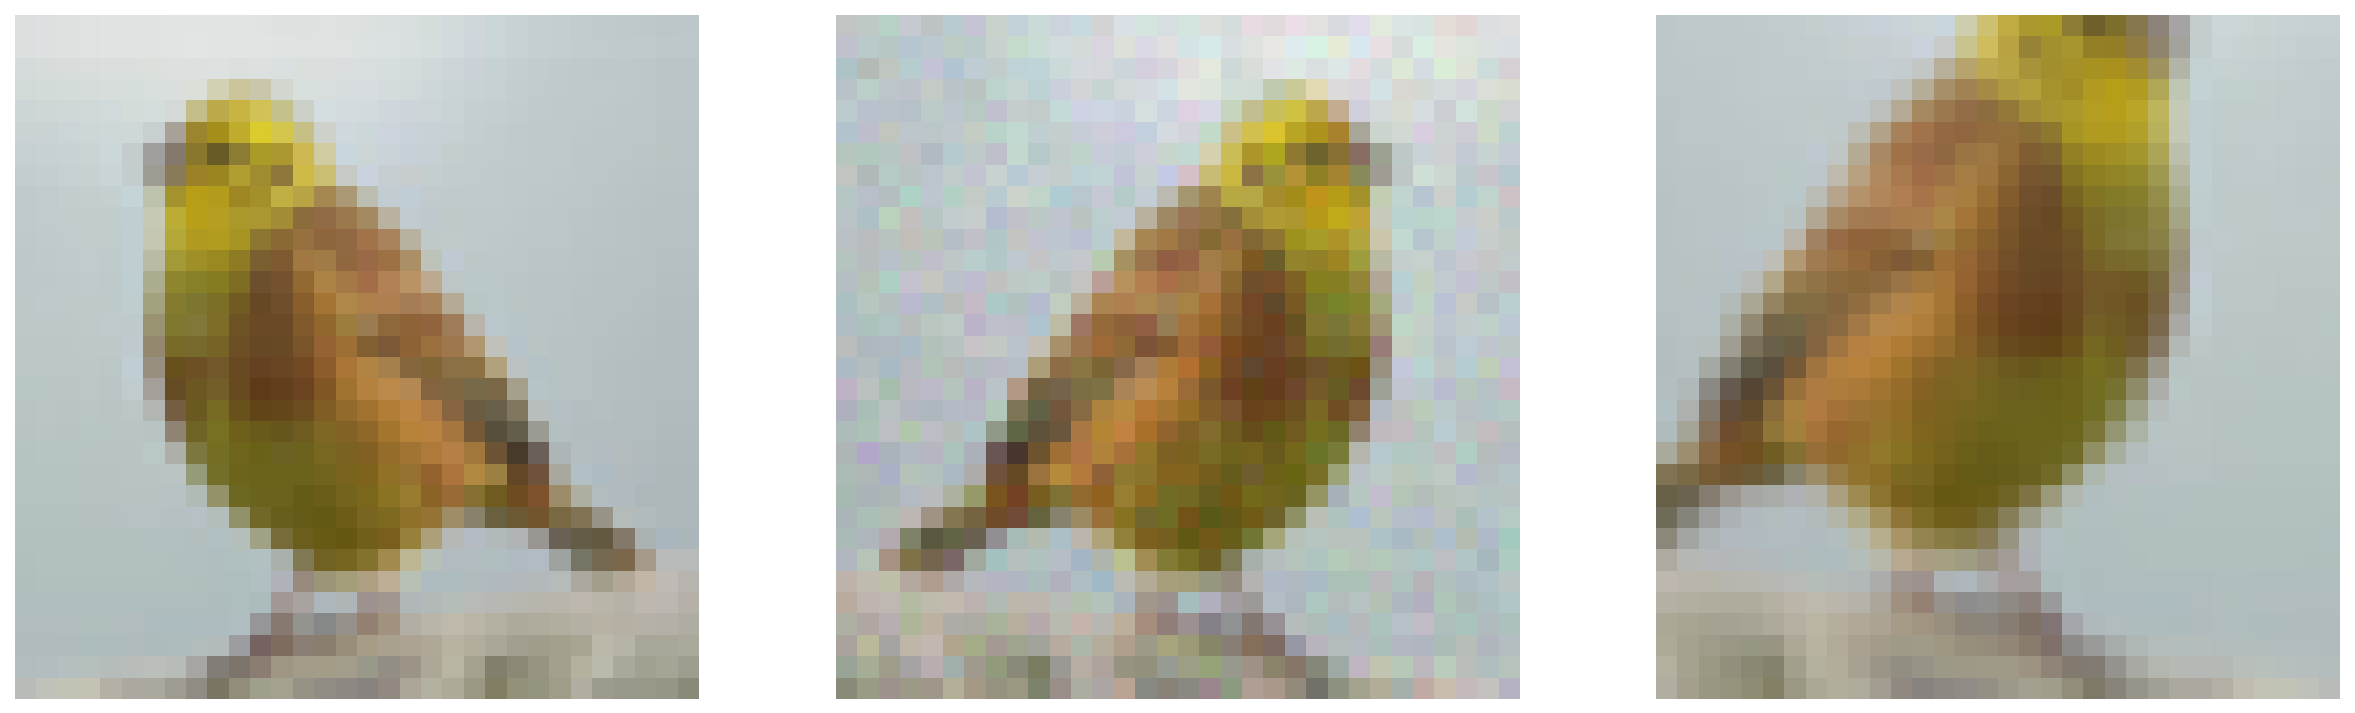
\includegraphics[width=\linewidth]{images/augmentation3.png}
        \caption{An example of augmentation applied on a CIFAR-10 32$\times$32 image using the "imgaug" Python libary [N] (ltr: flip, gaussian noise, crop)}
        \label{fig:augmentation}
\end{figure}

Another way to try to compensate for class imbalance is by doing \emph{oversampling} [N] where the model gets fed samples of the minority classes more often.
%Even though \emph{undersampling} (the deletion of samples of big classes) is also an option in extreme cases, this method shows no reason to have a positive impact on learnability imbalance.
%This is because the aim is to increase the true positive rates of harder to learn classes, which will most likely not happend by reducing the other classes. 
%It will rather just reduce the accuracy of 

Even though \emph{undersampling} (the ignoring of samples of big classes) is also an option in extreme cases, it is more likely to have an negative impact on the learnability imbalance.
That's because, when reducing the size of easier to learn classes, it will probably result in the decrease of their accuracy without an increase of the accuracy of the other classes.
This hypothesis will also be checked in this research.

From the approaches mentioned above, the focal loss is the only one that can be tested on balanced datasets as it is. 
The others require a pre-training in order to determine the learnability differences and therefore the true positive rates, which then can be used to estimate or calculate how much these methods should affect each class.






%When working with unbalanced datasets this 
%\[ \text{L}(x, c) = w_{c} \left(-y_{c} \cdot \log\left(N(x, \theta)\right) \right) \]


%The formula 1 above represents the weighted cross entropy loss where $x$ is an input sample and $y_{class}$ the integer representation of the corresponding class with $y := \{0, ..., C-1\}$.
%$N(x, \theta)$ is the output of the model with the learnable parameters $\theta$ and can be described by a probablity distribution $P(y|x,\theta)$. $P(y_{class}|x,\theta)$ represents the confidence of the model that sample $x$ corresponds to class $class$ with the property $\sum_{i=0}^{C-1}P(y_i|x,\theta) = 1$.
%$\left|N(x, \theta)\right| = C$ is the probablity distribution calculated using the learnable parameters $\theta$.
%The output $P(x|\theta) = N(x, \theta)$ is a probablity distribution with $\left|N(x, \theta)\right| = C$  $P(x = i|\theta)$ is the probablity that the input $x$ corresponds to class $i$.

\section{methodology}
In order to produce appropriate results, the proposed approach has to be applied on different models with different tasks. 
There are three main diciplines: image, sequential data and tabular data classification. 
When testing the approach on each task, the results can be interpreted more generalized. 
But it can also reveal if it works better for one specific dicipline than for others. 
If there is such a suspicion, the methods can be testes on more datasets of such diciplines.

As already presented in the introduction, the approach will be tested on the CIFAR-10 dataset for image classification.
It contains 60.000 32$\times$32 pixel RGB (i.e. channels for red, green and blue color) images, that are equally distributed among ten classes.
This dataset is freely available and commonly used in computer vision research.
The model architecture of the model will be a tradionional convolutional neural network [N] with residual connections [N].
For testing the approach on sequential data, a name-ethnicity dataset will be used.
This dataset was gathered by the government of United Kindom Of Great Britain and provided to one of the authors for a prior collaboration project based on name-ethnicity-classification.
Within this research the maximum accuracy for this classification problem was reached by using a \emph{ConvLSTM} architecture [N], i.e. the combination of a convolutional neural network and a LSTM (long-short term memory) [N], which will also be used in this research. 
Finally, the tabular dataset that will be used is the ------ dataset which contains of --------------- with --- classes.

%The metric used to measure the effectiveness of the approach will be the difference of the variance of the per-class accruacies produced when training with weighting augmentation and without.
The metric used for measuring how much a potential learnability imbalance impacted the model is the variance of the per-class accuracies.
Therefore, the effectiveness of the proposed approach can be determined by the difference between the variances generated with and without the approach.

\[ Var(s) = \frac{1}{C} \sum_{i=1}^{C} (s_i - \bar{s})^2 \]
\[ D = Var(s) - Var(s') \]

$s'$ are the true positive scores produced by a model using one of the proposed methods and $s$ of a model that was trained normally. 
If $Var(s')$ is smaller that $Var(s)$, the approach showed a potential effectiveness.
But if the difference is not significant, a staistical test must be performed in order to be sure that the reason for this difference was indeed the method.

The experiments will be implemented in the \emph{Python} programming language and the models will be built and trained using the \emph{Pytorch} deep learning framework [N].
In addition, an experiment manager, such as \emph{Weights\&Baises} [N], keeps the results in an orderly and accessible manner.

%Further, all experiments will be performed using \emph{cross validation} [N].
%That means that the dataset will be split into $K$ parts of which one is used for evaluating and the rest for training the neural network.
%When the dataset is split randomly into two parts, the results of the model are dependent of the data it was trained on.
%To be sure of the models results, it will be trained $K$ times independently and finally the evaluation scores will be averaged along all $K$ results.
%In order to be sure, that the results are not good or bad because an unfortunate split of the dataset.

\section{research plan}
This research is expected to be completed in a short period and not consume many ressources.
The reason for that is that the capacities (i.e. number of parameters) of the models used for the experiments are not high, since they don't need to reach state-of-the-art results.
Additionally, since the datasets (which are already provided) are not particularly high dimensional, the experiments do not require high-end hardware and can be run in a short amount of time.

The esitmated duration of this research is 13 months and will be performed in four stages, as shown in the table below.

\begin{center}
        \captionof{table}{schedule of research} 

        \begin{tabular}{ |c|c|c|c| } 
                \hline
                stage & description & duration \\
                \hline
                %\multirow{3}{4em}{Multiple row} & cell2 & cell3 \\ 
                1 & investigation & 4 months \\ 
                2 & execution & 6 months \\ 
                3 & revision & 2 months \\ 
                4 & writing & 3 months \\
                \hline

        \end{tabular}
\end{center}
        
In the first stage, the investigation, theoretical approaches are conceptualized by doing a more indepth literature review and adapting the proposed approaches to the learnablity imbalance problem. 
The aim is to find several candidates for functions that produce loss weights, augmentation chances and oversampling amounts based on the true positive scores.
This investigation gives also the opportunity to encounter previously unconsidered methods with which the research can be extended.

The execution stage will begin by setting up the project code repository (link [N]). 
It will contain the model architectures, train scripts and implementations of the conceived methods.
Then the experiments will be run, the results collected and finally analyzed. 

In the next stage, the revision, the used approaches and the results will be reviewed and compared. 
After this process is finished, the last stage, the writing of the research paper can begin. 
Presumably after three months, the paper can be submitted and is ready for reviewing. 

\section{conclusion} 
TODO fourth section here

\begin{thebibliography}{1}

\bibitem{}
Name Name, Name Name, Name Name (2006). Title, 24(1), 29-33.

\end{thebibliography}

\end{document}

% biased class distribution: https://link.springer.com/chapter/10.1007/3-540-44795-4_45#:~:text=Labeled%20data%20for%20classification%20could,optimal%20classification%20on%20new%20data.
% class imbalance over sampling: https://machinelearningmastery.com/random-oversampling-and-undersampling-for-imbalanced-classification/
% CEL: https://arxiv.org/ftp/arxiv/papers/2001/2001.00570.pdf
% a: https://arxiv.org/pdf/1901.05555.pdf (p 4)
% focal loss: https://arxiv.org/pdf/1708.02002.pdf
% smote: https://arxiv.org/pdf/1106.1813.pdf